
%% bare_conf.tex
%% V1.3
%% 2007/01/11
%% by Michael Shell
%% See:
%% http://www.michaelshell.org/
%% for current contact information.
%%
%% This is a skeleton file demonstrating the use of IEEEtran.cls
%% (requires IEEEtran.cls version 1.7 or later) with an IEEE conference paper.
%%
%% Support sites:
%% http://www.michaelshell.org/tex/ieeetran/
%% http://www.ctan.org/tex-archive/macros/latex/contrib/IEEEtran/
%% and
%% http://www.ieee.org/

%%*************************************************************************
%% Legal Notice:
%% This code is offered as-is without any warranty either expressed or
%% implied; without even the implied warranty of MERCHANTABILITY or
%% FITNESS FOR A PARTICULAR PURPOSE! 
%% User assumes all risk.
%% In no event shall IEEE or any contributor to this code be liable for
%% any damages or losses, including, but not limited to, incidental,
%% consequential, or any other damages, resulting from the use or misuse
%% of any information contained here.
%%
%% All comments are the opinions of their respective authors and are not
%% necessarily endorsed by the IEEE.
%%
%% This work is distributed under the LaTeX Project Public License (LPPL)
%% ( http://www.latex-project.org/ ) version 1.3, and may be freely used,
%% distributed and modified. A copy of the LPPL, version 1.3, is included
%% in the base LaTeX documentation of all distributions of LaTeX released
%% 2003/12/01 or later.
%% Retain all contribution notices and credits.
%% ** Modified files should be clearly indicated as such, including  **
%% ** renaming them and changing author support contact information. **
%%
%% File list of work: IEEEtran.cls, IEEEtran_HOWTO.pdf, bare_adv.tex,
%%                    bare_conf.tex, bare_jrnl.tex, bare_jrnl_compsoc.tex
%%*************************************************************************

% *** Authors should verify (and, if needed, correct) their LaTeX system  ***
% *** with the testflow diagnostic prior to trusting their LaTeX platform ***
% *** with production work. IEEE's font choices can trigger bugs that do  ***
% *** not appear when using other class files.                            ***
% The testflow support page is at:
% http://www.michaelshell.org/tex/testflow/



% Note that the a4paper option is mainly intended so that authors in
% countries using A4 can easily print to A4 and see how their papers will
% look in print - the typesetting of the document will not typically be
% affected with changes in paper size (but the bottom and side margins will).
% Use the testflow package mentioned above to verify correct handling of
% both paper sizes by the user's LaTeX system.
%
% Also note that the "draftcls" or "draftclsnofoot", not "draft", option
% should be used if it is desired that the figures are to be displayed in
% draft mode.
%
\documentclass[10pt, conference]{IEEEtran}
% Add the compsocconf option for Computer Society conferences.
%
% If IEEEtran.cls has not been installed into the LaTeX system files,
% manually specify the path to it like:
% \documentclass[conference]{../sty/IEEEtran}





% Some very useful LaTeX packages include:
% (uncomment the ones you want to load)


% *** MISC UTILITY PACKAGES ***
%
%\usepackage{ifpdf}
% Heiko Oberdiek's ifpdf.sty is very useful if you need conditional
% compilation based on whether the output is pdf or dvi.
% usage:
% \ifpdf
%   % pdf code
% \else
%   % dvi code
% \fi
% The latest version of ifpdf.sty can be obtained from:
% http://www.ctan.org/tex-archive/macros/latex/contrib/oberdiek/
% Also, note that IEEEtran.cls V1.7 and later provides a builtin
% \ifCLASSINFOpdf conditional that works the same way.
% When switching from latex to pdflatex and vice-versa, the compiler may
% have to be run twice to clear warning/error messages.






% *** CITATION PACKAGES ***
%
%\usepackage{cite}
% cite.sty was written by Donald Arseneau
% V1.6 and later of IEEEtran pre-defines the format of the cite.sty package
% \cite{} output to follow that of IEEE. Loading the cite package will
% result in citation numbers being automatically sorted and properly
% "compressed/ranged". e.g., [1], [9], [2], [7], [5], [6] without using
% cite.sty will become [1], [2], [5]--[7], [9] using cite.sty. cite.sty's
% \cite will automatically add leading space, if needed. Use cite.sty's
% noadjust option (cite.sty V3.8 and later) if you want to turn this off.
% cite.sty is already installed on most LaTeX systems. Be sure and use
% version 4.0 (2003-05-27) and later if using hyperref.sty. cite.sty does
% not currently provide for hyperlinked citations.
% The latest version can be obtained at:
% http://www.ctan.org/tex-archive/macros/latex/contrib/cite/
% The documentation is contained in the cite.sty file itself.






% *** GRAPHICS RELATED PACKAGES ***
%
\ifCLASSINFOpdf
  % \usepackage[pdftex]{graphicx}
  % declare the path(s) where your graphic files are
  % \graphicspath{{../pdf/}{../jpeg/}}
  % and their extensions so you won't have to specify these with
  % every instance of \includegraphics
  % \DeclareGraphicsExtensions{.pdf,.jpeg,.png}
\else
  % or other class option (dvipsone, dvipdf, if not using dvips). graphicx
  % will default to the driver specified in the system graphics.cfg if no
  % driver is specified.
  % \usepackage[dvips]{graphicx}
  % declare the path(s) where your graphic files are
  % \graphicspath{{../eps/}}
  % and their extensions so you won't have to specify these with
  % every instance of \includegraphics
  % \DeclareGraphicsExtensions{.eps}
\fi
% graphicx was written by David Carlisle and Sebastian Rahtz. It is
% required if you want graphics, photos, etc. graphicx.sty is already
% installed on most LaTeX systems. The latest version and documentation can
% be obtained at: 
% http://www.ctan.org/tex-archive/macros/latex/required/graphics/
% Another good source of documentation is "Using Imported Graphics in
% LaTeX2e" by Keith Reckdahl which can be found as epslatex.ps or
% epslatex.pdf at: http://www.ctan.org/tex-archive/info/
%
% latex, and pdflatex in dvi mode, support graphics in encapsulated
% postscript (.eps) format. pdflatex in pdf mode supports graphics
% in .pdf, .jpeg, .png and .mps (metapost) formats. Users should ensure
% that all non-photo figures use a vector format (.eps, .pdf, .mps) and
% not a bitmapped formats (.jpeg, .png). IEEE frowns on bitmapped formats
% which can result in "jaggedy"/blurry rendering of lines and letters as
% well as large increases in file sizes.
%
% You can find documentation about the pdfTeX application at:
% http://www.tug.org/applications/pdftex





% *** MATH PACKAGES ***
%
%\usepackage[cmex10]{amsmath}
% A popular package from the American Mathematical Society that provides
% many useful and powerful commands for dealing with mathematics. If using
% it, be sure to load this package with the cmex10 option to ensure that
% only type 1 fonts will utilized at all point sizes. Without this option,
% it is possible that some math symbols, particularly those within
% footnotes, will be rendered in bitmap form which will result in a
% document that can not be IEEE Xplore compliant!
%
% Also, note that the amsmath package sets \interdisplaylinepenalty to 10000
% thus preventing page breaks from occurring within multiline equations. Use:
%\interdisplaylinepenalty=2500
% after loading amsmath to restore such page breaks as IEEEtran.cls normally
% does. amsmath.sty is already installed on most LaTeX systems. The latest
% version and documentation can be obtained at:
% http://www.ctan.org/tex-archive/macros/latex/required/amslatex/math/





% *** SPECIALIZED LIST PACKAGES ***
%
%\usepackage{algorithmic}
% algorithmic.sty was written by Peter Williams and Rogerio Brito.
% This package provides an algorithmic environment fo describing algorithms.
% You can use the algorithmic environment in-text or within a figure
% environment to provide for a floating algorithm. Do NOT use the algorithm
% floating environment provided by algorithm.sty (by the same authors) or
% algorithm2e.sty (by Christophe Fiorio) as IEEE does not use dedicated
% algorithm float types and packages that provide these will not provide
% correct IEEE style captions. The latest version and documentation of
% algorithmic.sty can be obtained at:
% http://www.ctan.org/tex-archive/macros/latex/contrib/algorithms/
% There is also a support site at:
% http://algorithms.berlios.de/index.html
% Also of interest may be the (relatively newer and more customizable)
% algorithmicx.sty package by Szasz Janos:
% http://www.ctan.org/tex-archive/macros/latex/contrib/algorithmicx/
\usepackage{amsmath}
\usepackage{centernot}
\usepackage{tikz}
\usepackage{xspace}

% *** ALIGNMENT PACKAGES ***
%
%\usepackage{array}
% Frank Mittelbach's and David Carlisle's array.sty patches and improves
% the standard LaTeX2e array and tabular environments to provide better
% appearance and additional user controls. As the default LaTeX2e table
% generation code is lacking to the point of almost being broken with
% respect to the quality of the end results, all users are strongly
% advised to use an enhanced (at the very least that provided by array.sty)
% set of table tools. array.sty is already installed on most systems. The
% latest version and documentation can be obtained at:
% http://www.ctan.org/tex-archive/macros/latex/required/tools/


%\usepackage{mdwmath}
%\usepackage{mdwtab}
% Also highly recommended is Mark Wooding's extremely powerful MDW tools,
% especially mdwmath.sty and mdwtab.sty which are used to format equations
% and tables, respectively. The MDWtools set is already installed on most
% LaTeX systems. The lastest version and documentation is available at:
% http://www.ctan.org/tex-archive/macros/latex/contrib/mdwtools/


% IEEEtran contains the IEEEeqnarray family of commands that can be used to
% generate multiline equations as well as matrices, tables, etc., of high
% quality.


%\usepackage{eqparbox}
% Also of notable interest is Scott Pakin's eqparbox package for creating
% (automatically sized) equal width boxes - aka "natural width parboxes".
% Available at:
% http://www.ctan.org/tex-archive/macros/latex/contrib/eqparbox/





% *** SUBFIGURE PACKAGES ***
%\usepackage[tight,footnotesize]{subfigure}
% subfigure.sty was written by Steven Douglas Cochran. This package makes it
% easy to put subfigures in your figures. e.g., "Figure 1a and 1b". For IEEE
% work, it is a good idea to load it with the tight package option to reduce
% the amount of white space around the subfigures. subfigure.sty is already
% installed on most LaTeX systems. The latest version and documentation can
% be obtained at:
% http://www.ctan.org/tex-archive/obsolete/macros/latex/contrib/subfigure/
% subfigure.sty has been superceeded by subfig.sty.



%\usepackage[caption=false]{caption}
%\usepackage[font=footnotesize]{subfig}
% subfig.sty, also written by Steven Douglas Cochran, is the modern
% replacement for subfigure.sty. However, subfig.sty requires and
% automatically loads Axel Sommerfeldt's caption.sty which will override
% IEEEtran.cls handling of captions and this will result in nonIEEE style
% figure/table captions. To prevent this problem, be sure and preload
% caption.sty with its "caption=false" package option. This is will preserve
% IEEEtran.cls handing of captions. Version 1.3 (2005/06/28) and later 
% (recommended due to many improvements over 1.2) of subfig.sty supports
% the caption=false option directly:
%\usepackage[caption=false,font=footnotesize]{subfig}
%
% The latest version and documentation can be obtained at:
% http://www.ctan.org/tex-archive/macros/latex/contrib/subfig/
% The latest version and documentation of caption.sty can be obtained at:
% http://www.ctan.org/tex-archive/macros/latex/contrib/caption/




% *** FLOAT PACKAGES ***
%
%\usepackage{fixltx2e}
% fixltx2e, the successor to the earlier fix2col.sty, was written by
% Frank Mittelbach and David Carlisle. This package corrects a few problems
% in the LaTeX2e kernel, the most notable of which is that in current
% LaTeX2e releases, the ordering of single and double column floats is not
% guaranteed to be preserved. Thus, an unpatched LaTeX2e can allow a
% single column figure to be placed prior to an earlier double column
% figure. The latest version and documentation can be found at:
% http://www.ctan.org/tex-archive/macros/latex/base/



%\usepackage{stfloats}
% stfloats.sty was written by Sigitas Tolusis. This package gives LaTeX2e
% the ability to do double column floats at the bottom of the page as well
% as the top. (e.g., "\begin{figure*}[!b]" is not normally possible in
% LaTeX2e). It also provides a command:
%\fnbelowfloat
% to enable the placement of footnotes below bottom floats (the standard
% LaTeX2e kernel puts them above bottom floats). This is an invasive package
% which rewrites many portions of the LaTeX2e float routines. It may not work
% with other packages that modify the LaTeX2e float routines. The latest
% version and documentation can be obtained at:
% http://www.ctan.org/tex-archive/macros/latex/contrib/sttools/
% Documentation is contained in the stfloats.sty comments as well as in the
% presfull.pdf file. Do not use the stfloats baselinefloat ability as IEEE
% does not allow \baselineskip to stretch. Authors submitting work to the
% IEEE should note that IEEE rarely uses double column equations and
% that authors should try to avoid such use. Do not be tempted to use the
% cuted.sty or midfloat.sty packages (also by Sigitas Tolusis) as IEEE does
% not format its papers in such ways.

\newif\ifdraft
\drafttrue

%\input{macros}



% *** PDF, URL AND HYPERLINK PACKAGES ***
%
\usepackage{url}
% url.sty was written by Donald Arseneau. It provides better support for
% handling and breaking URLs. url.sty is already installed on most LaTeX
% systems. The latest version can be obtained at:
% http://www.ctan.org/tex-archive/macros/latex/contrib/misc/
% Read the url.sty source comments for usage information. Basically,
% \url{my_url_here}.





% *** Do not adjust lengths that control margins, column widths, etc. ***
% *** Do not use packages that alter fonts (such as pslatex).         ***
% There should be no need to do such things with IEEEtran.cls V1.6 and later.
% (Unless specifically asked to do so by the journal or conference you plan
% to submit to, of course. )


% correct bad hyphenation here
\hyphenation{op-tical net-works semi-conduc-tor}


\begin{document}
%
% paper title
% can use linebreaks \\ within to get better formatting as desired
\title{Locating the buggy version based on a bisection test idea. Two case of studies: ElasticSearch and Nova}


% author names and affiliations
% use a multiple column layout for up to two different
% affiliations

\author{\IEEEauthorblockN{Gema Rodriguez-Perez}
\IEEEauthorblockA{LibreSoft/GSyC\\
Universidad Rey Juan Carlos\\
Fuenlabrada, Spain\\
gerope@libresoft.info}
\and
\IEEEauthorblockN{Gregorio Robles}
\IEEEauthorblockA{LibreSoft/GSyC\\
Universidad Rey Juan Carlos\\
Fuenlabrada, Spain\\
grex@gsyc.urjc.es}
\and
\IEEEauthorblockN{Jesus M. Gonzalez-Barahona}
\IEEEauthorblockA{LibreSoft/GSyC\\
Universidad Rey Juan Carlos\\
Fuenlabrada, Spain\\
jgb@gsyc.es}
}

% conference papers do not typically use \thanks and this command
% is locked out in conference mode. If really needed, such as for
% the acknowledgment of grants, issue a \IEEEoverridecommandlockouts
% after \documentclass

% for over three affiliations, or if they all won't fit within the width
% of the page, use this alternative format:
% 
%\author{\IEEEauthorblockN{Michael Shell\IEEEauthorrefmark{1},
%Homer Simpson\IEEEauthorrefmark{2},
%James Kirk\IEEEauthorrefmark{3}, 
%Montgomery Scott\IEEEauthorrefmark{3} and
%Eldon Tyrell\IEEEauthorrefmark{4}}
%\IEEEauthorblockA{\IEEEauthorrefmark{1}School of Electrical and Computer Engineering\\
    %Georgia Institute of Technology,
%Atlanta, Georgia 30332--0250\\ Email: see http://www.michaelshell.org/contact.html}
%\IEEEauthorblockA{\IEEEauthorrefmark{2}Twentieth Century Fox, Springfield, USA\\
%Email: homer@thesimpsons.com}
%\IEEEauthorblockA{\IEEEauthorrefmark{3}Starfleet Academy, San Francisco, California 96678-2391\\
%Telephone: (800) 555--1212, Fax: (888) 555--1212}
%\IEEEauthorblockA{\IEEEauthorrefmark{4}Tyrell Inc., 123 Replicant Street, Los Angeles, California 90210--4321}}




% use for special paper notices
%\IEEEspecialpapernotice{(Invited Paper)}




% make the title area
\maketitle


\begin{abstract}
Many studies in the software research literature on bug fixing are built upon the assumption that “a given bug was introduced by the lines of code that were modified to fix it”, or variations of it. Although this assumption seems at first glance very reasonable, there is little empirical evidence supporting it. But a careful examination surfaces many other possible sources for the introduction of bugs, from previous modifications to those lines, to changes completely external to the piece of code being considered. In this paper we have explored carefully how a number of bugs were introduced in two different software projects, with the intention of better understanding the complex phenomenon of bug introduction and bug fixing. From this observation, we have developed a comprehensive model of how bugs are introduced, including
definitions and a taxonomy which help to analyze formally the process. The taxonomy helps to understand the many different ways in which a bug is introduced, and why some of the methods proposed in the literature fail to find many of them. The model allows as well for a better framing of the comparison of automatic methods to find bug inducting changes, which we apply to analyze some of these methods. Finally, based on this comparison, we propose some method that at least in the cases considered show better results than
the classical methods described in the literature.


\end{abstract}

\begin{IEEEkeywords}
Bug introduction change; bug seeding metrics;

\end{IEEEkeywords}


% For peer review papers, you can put extra information on the cover
% page as needed:
% \ifCLASSOPTIONpeerreview
% \begin{center} \bfseries EDICS Category: 3-BBND \end{center}
% \fi
%
% For peerreview papers, this IEEEtran command inserts a page break and
% creates the second title. It will be ignored for other modes.
\IEEEpeerreviewmaketitle



\section{Introduction}
\label{sec:intro}

%When a failure is found in some software, developers usually fix it by locating and modifying the source code line(s) that are the cause for the wrong behavior. It seems reasonable to assume that the immediately previous modifications of these lines are the cause of the bug. However, finding where and when a bug was introduced in the source code is not a trivial task, and it may be much more complex than what this assumption suggests.
Fixing a bug in a software component usually consists of determining why it is behaving erroneously, and then correcting the source code that causes that erroneous behavior. That is, the developer fixing the bug produces a change to the source code, which can be clearly identified as the bug-fixing change. Identifying which change or changes to the code introduced the bug for the first time is another story, which when analyzed in detail, proves to be, in many cases, difficult to tell.

Previous work of Silwerski, Zimmermann, and Zeller were successfully able to identify changes in version control that induced fixes of bugs creating the well-known algorithm SZZ\cite{sliwerski2005changes}. However, we know that exists certain common change patterns that occur in the normal development process that make this method less useful, such as an older modification, or a change in some API in a different part of the code. Thus, this causes issues when you attempt to identify the location of the bug by assuming that the last modification to change that particular line has injected the buggy line.

To mitigate the false positives that such algorithm causes, we believe in the idea that version control system bisection provides. Hence an issue is resolved and a test case is added in a revision, we might know that the bug have been injected before that revision. Thus, going back to previous revisions and testing the software we might determine whether or not the bug is present. If it is indeed present, the test case fails and the bug must have been injected before (or by) that revision. In our work and base on this idea, we have used information from the source code management system, the issue tracking system and the code review system to first understand which was the malfunction caused by the bug, what problems in the source code were causing it, and how it was finally fixed. Empowered with all these data, we have navigated back in the history of the software component, to find out when the malfunction was happening for the first time, and which change or changes to the code, if any, introduced that malfunction.

This paper tries to present two main contributions, one the one hand, a manual analysis of two Open Source projects (ElasticSearch and Nova) to locate when the malfunction happened base on the idea of an hypothetical test which checks the current version of the software assuming it as stable version that either passes or not the test. In this analysis, we use two different techniques to analyze the source code, one base at line level while the other is base at token level. Furthermore, the outcome provides by this analysis causes a comparison with the results of SZZ algorithm in the same data set. As well as, once we know exactly the moment of the malfunction we are able to calculate metrics such as the Time To Fix (TTF), the Time To Review (TTR), the Time To Notify (TTN) a bug or the fix-effort to improve code quality.

One the other hand, we would like to contribute to current literature with a systematic review about the credibility of the most popular algorithm used to identify induced fixes mentioned before, the SZZ algorithm \cite{sliwerski2005changes}. Because many studies in the area of software maintenance and evolution start with the implicit assumption that this algorithm used, in which the line (or lines) that is being replaced in a bug fix is likely the one that created such bug. Thus, our goal is to attempt to guide practitioners and teach some of the lessons learned to mitigate the issues that this algorithm causes in fields such as bug detection or bug prediction. 

\section{Finding the origins of a Bug}
\label{sec:finding}

This section describes the methodology that we used in our empirical experiment to find the origin of the malfunction in the software using the token method and the line method. In the case of Nova and ElasticSearch, the data needed can be obtained from the source code management, issue tracking system, and code review system. We had followed the next methodology for the line method and the token method.

Figure~\ref{fig:diagram} provides an overview of each step involved in our study and their outcomes.

\begin{figure}[ht]
\centering
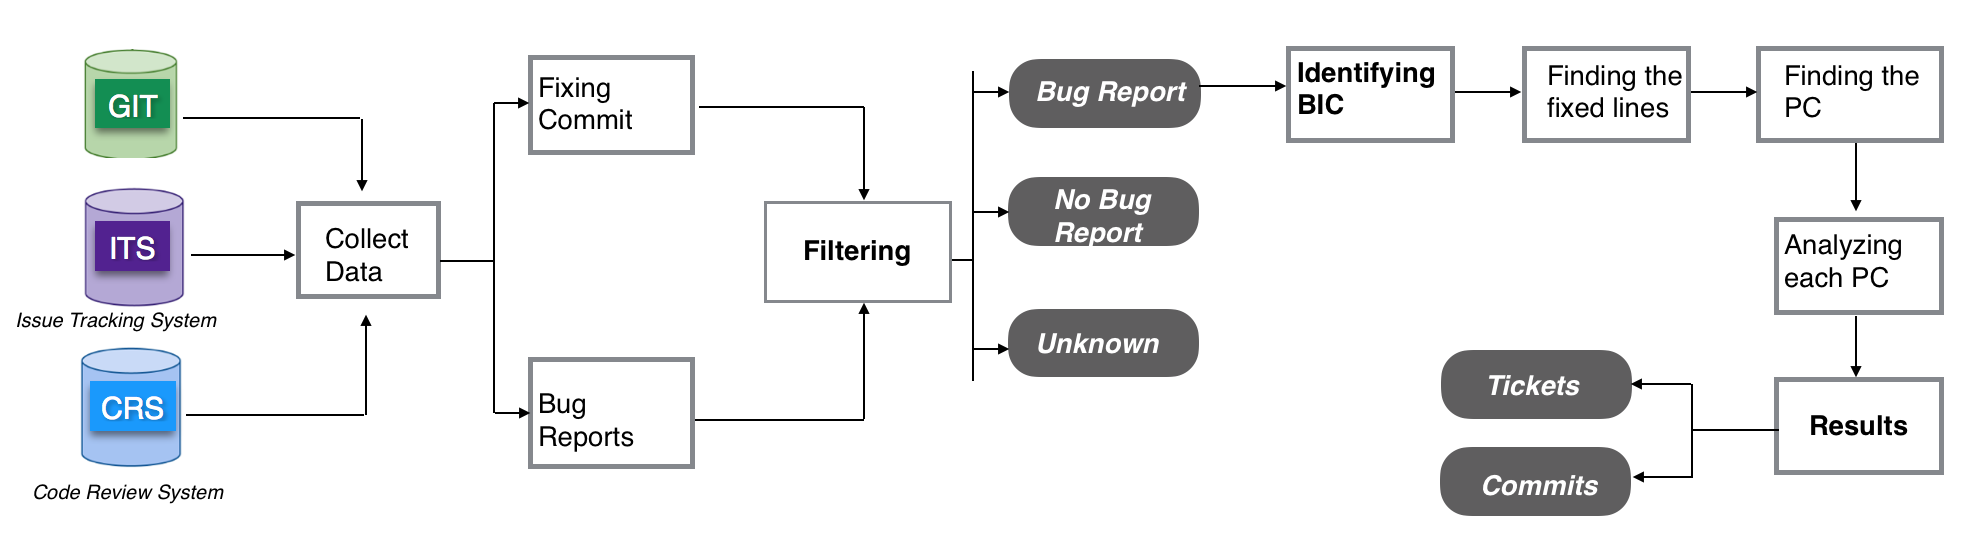
\includegraphics[width=\columnwidth]{diagram.png}
\caption{Overview of the steps involved in our analysis }
\label{fig:diagram}       % Give a unique label
\end{figure}

\subsection{Identifying the Bug introducing change of a ticket}
\label{sec:methodologySS}
The income of this stage is a set of bug report tickets extracted randomly from the issue tracking system. All of these tickets have to have been closed and have a fixed commit committed and merged in the code source of the project to be able to follow the methodology described at this section.

\subsubsection{Finding the fixed lines of the bug}
We identify the commit that fixed the bug from the information of the bug fix commit, finding the line(s)/token(s) that this commit added, modified or deleted and filtering out line(s)/token(s) that are not the code.
	
\subsubsection{Finding the previous commit of that lines/tokens}

Each line/token touched by the bug fix commit has only one immediately previous commit, we will refer to such commits as $pc$. This $pc$ could be the same or could be different in such line(s)/token(s). The result of this is a set of all $pc$ of the bug.

\subsubsection{Analyzing each previous commits }

This analysis uses information from the bug fix commit log and the ticket description, as well as from the log and commit changes of the $pc$ and also from the history version of each changed line/token. In this analysis, we use the idea of an hypothetical test which checks the current version of the software assuming it as stable version that either passes or not the test.

Figure~\ref{fig:test} shows the check test idea. Considering that we have an omnipotent view, we can find the candidate to be the $BIC$ of a bug. The test is passed to all previous commits looking for the one that fails; if found, we will be consider it as a candidate for the $BIC$. However, to be sure about the commit being the $BIC$, we have to check that the line(s)/token(s) inserted by this commit was (were) buggy, otherwise it can not be considered as the $BIC$.

\begin{figure}[ht]
\centering
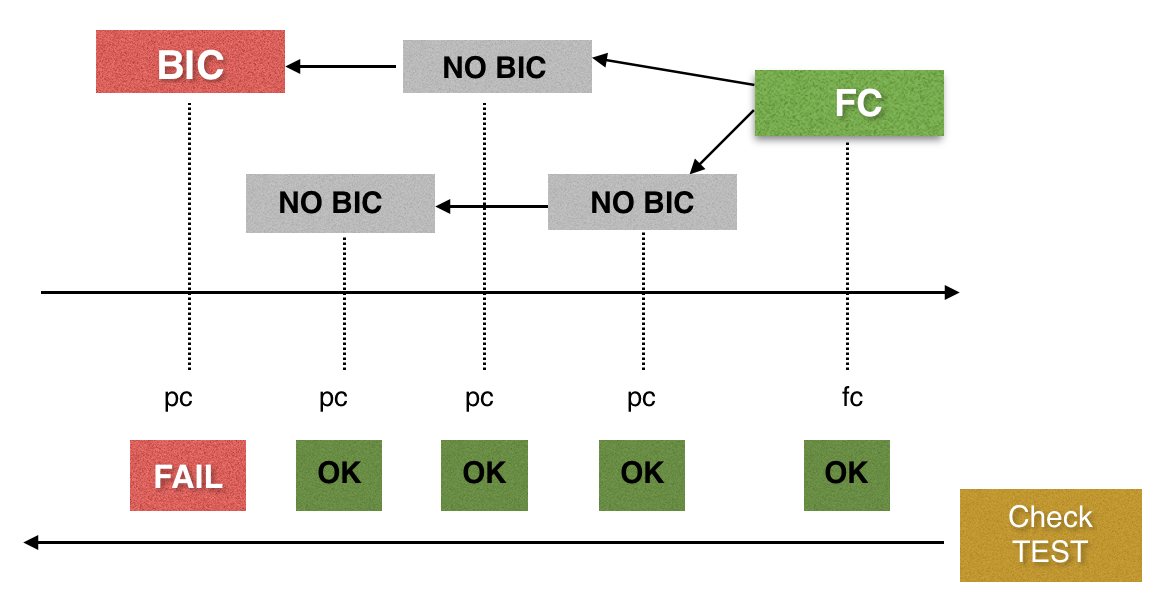
\includegraphics[width=\columnwidth]{testrecursive.png}
\caption{Example of how we could find a candidate commit to be the $BIC$. Each version passes or not a test written after fixing the bug in the FC (fixing commit).}
\label{fig:test}      
\end{figure}

At the end of this step we have two main groups for each bug analyzed:
\begin{itemize}
	\item Group 1 : The bug has been always there, then the test will always fail.
	\item Group 2: The bug can be found using the test. Thus, we have two main reasons: (a) The test fails as we expected because the failure was due to a change in other part of the code that affects the code fixed or  the fixed line(s)/token(s) cannot be checked before because they didn't exists. (b) The test fails because a previous change (the $ipc$ or an older commit) injected the bug.
\end{itemize}

\subsection{results}

We have analyzed 59 random bug reports from the two projects, determining the origin of a bug. Thus, after finding the line(s)/token(s) which fix the bug in the 59 bug reports we found that almost   

\begin{table}[!t]
\renewcommand{\arraystretch}{1.3}
\caption{Number of previous commit per ticket in each of the two projects analyzed, line level}
\label{tableI}
\centering
\begin{tabular}{|c||c||c|c|c|}
\hline
 & Nova(L) & ES(L)& Nova(T) & ES(T) \\
\hline
Group 1 & 7(12\%) & 19(32\%)& 7(12\%) & 16(27\%)\\
\hline
Group 2(a) & 29 (49\%) & 18 (31\%)& 33 (56\%) & 24 (40\%)\\
\hline
Group 2(b) & 23 (39\%) & 22(37\%)& 19(32\%) & 19(32\%)\\
\hline
\end{tabular}
\end{table}

The number of commits analyzed at line level was --- in Nova and -- in ElasticSearch, in the 90\% of the cases the SZZ algorithm was able to find them in both projects. But, from the 90\% of commits founded, only in 45\% in Nova and 48\% in ElasticSearch the SZZ algorithm blame the correct $ipc$ as the cause of the bug.

On the other hand, the number of commits analyzed at token level was --- in both projects, between the 85-87\% of the cases the SZZ algorithm was able to find them. But, from the 85\% of commits founded, only in 48\% in Nova and 36\% in ElasticSearch the SZZ algorithm blame the correct $ipc$ as the cause of the bug. Some of the $ipc$ were classified into unknown set when we were no sure about whether it was a cause of the bug or not.

Additionally, in those cases where the test fails as we expected and the ticket does not present any BIC into the previous commits, we are able to present a short classification of the main reasons:
\begin{itemize}
  \item Changes to APIs, such as the addition of an argument. 
  \item Updates done, such as changes in the operating system, packages or requirements.
\end{itemize}

Furthermore, our research shows evidence that assuming that the $ipc$ is where the cause of a bug can be found does not hold for a significant fraction of bugs. The most common reasons for the $ipc$ was not a BIC in the projects are:

\begin{itemize}
  \item Variable renaming.
  \item Changes done by the bug fixing commit in a clean line.
  \item Refactoring of the code in some lines.
  \item Grammar errors, dragged from former commits.
\end{itemize} 

\section{metrics}
\label{sec:metrics}

To compute the metrics used in this study, we need to identify the BIC. Once this has been done, we are able to measure the time values. Next, we describe the metrics used in our study: 

\begin{itemize}
		\item \emph{Experience until Bug Introducing Change} (EuBIC): Experience of the author of the BIC at the moment of doing the commit. Experience is measured in days from the first time that the author committed some code to the project until the BIC.
		\item \emph{Time To Notify} (TTN): Time in days since the bug introducing commit was merged into the master branch until some developer notified the unexpected behavior and reported it in the bug tracking system. 
		\item \emph{Time To Fix} (TTF): Period in days from the notification of a bug report to when it was closed with a fixing commit.
		\item \emph{Bug Fixing Time} (BFT): Time in days from the date of the BIC to the fixing commit date. This value can be also computed by adding TTN and TTF.
\end{itemize} 

Figure~\ref{fig:metrics} provides a visual explanation of the metrics proposed in this paper. For example, to obtain the metrics for bug report, we need to identify the fixing commit and the BIC. Then, analyzing the meta-data of theses commits, we obtain the date and the author for both of them.

\begin{figure}[ht]
\centering
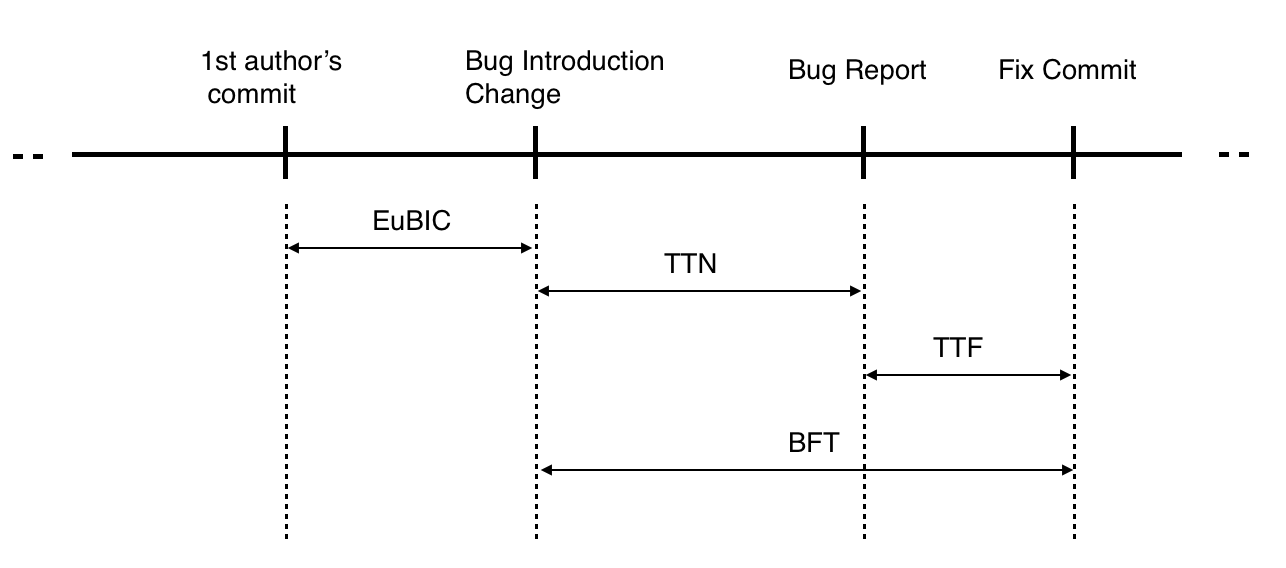
\includegraphics[width=\columnwidth]{metrics.png}
\caption{Visualization of the periods under study: Experience Until Bug Introducing Change (EuBIC),  Time To Notify (TTN), Time To Fix (TTF), Bug Fixing Time (BFT).}
\label{fig:metrics}       % Give a unique label
\end{figure}

We would like to compare our metrics with the widely used SZZ algorithm. We will therefore assume that the closest commit in time (i.e., the previous one) of the SZZ algorithm is the one that induces the bug-fixing commit, as it has been done in previous works~\cite{eyolfson2011time}. It should be noted, however, that the SZZ algorithm may not identify the BIC correctly, as its outcome could be a set of commits among which the \emph{real} BIC is not included. In addition, in our comparison we discard those fixing commits with only new lines, since the SZZ algorithm removes them from the analysis.

\subsection{results}

We have calculated the values of TTN, EuBIC and TTF for 76 bug fixing commits, 39 belonging to Nova and 37 belonging to ElasticSearch. 

Table~\ref{tableNova} and Table~\ref{tableES} show the means of Time To Notify (TTN), Time To Fix (TTF) and Bug Fixing Time (BFT) computed for the Nova and the ElasticSearch projects, respectively. The tables include the values for the \emph{real} BIC (manually checked), and the ones that can be obtained by using the SZZ algorithm.

\begin{table}[!t]
\renewcommand{\arraystretch}{1.3}
\centering
\caption{Mean in days of TTN, TTF, BFT for the Nova project, both for the \emph{real} BIC as for the BIC obtained with SZZ}
\label{tableNova}
\begin{tabular}{|c||c||c||c| }
\hline
  & TTN & TTF & BFT \\
\hline
Real & 432 & 65 & 497 \\
\hline
SZZ & 260 & 52 & 312\\
\hline
\end{tabular}
\end{table}

\begin{table}[!t]
\renewcommand{\arraystretch}{1.3}
\centering
\caption{Mean in days of TTN, TTF, BFT for the ElasticSearch project, both for the \emph{real} BIC as for the BIC obtained with SZZ.}
\label{tableES}
\begin{tabular}{|c||c||c||c| }
\hline
  & TTN & TTF & BFT \\
\hline
Real & 312 & 14 & 326 \\
\hline
SZZ & 135 & 16 & 151\\
\hline
\end{tabular}
\end{table}

In addition, Figure~\ref{fig:meansOfNova} and Figure~\ref{fig:meansOfES} show the values of TTN, TTF and EuBIC for both projects using box plots. We can see that it takes 158 days in ElasticSearch to notify 50\% of the bugs, and 336 days for Nova. The mean is almost 200 days in ElasticSearch and around 350 days in Nova. TTF is low for both projects, but especially for ElasticSearch where there is almost no dispersion and bugs are fixed almost immediately after their notification. And Nova developers are slightly more experienced than ElasticSearch developers when they introduce bugs.

\begin{figure}[ht]
\centering
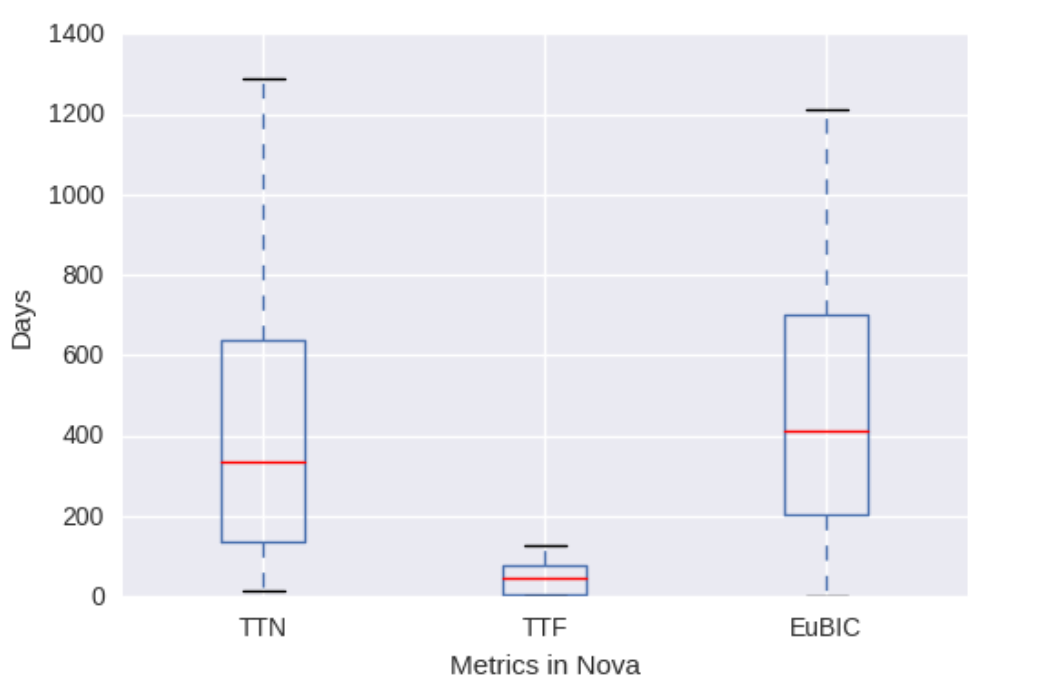
\includegraphics[width=\columnwidth]{boxplotNova.png}
\caption{Box-plots with TTN, TTF and EuBIC for the Nova project.}
\label{fig:meansOfNova}       % Give a unique label
%\caption{Box-Plot in Nova}
%\label{fig:graph4}       % Give a unique label
\end{figure}

\begin{figure}[ht]
\centering
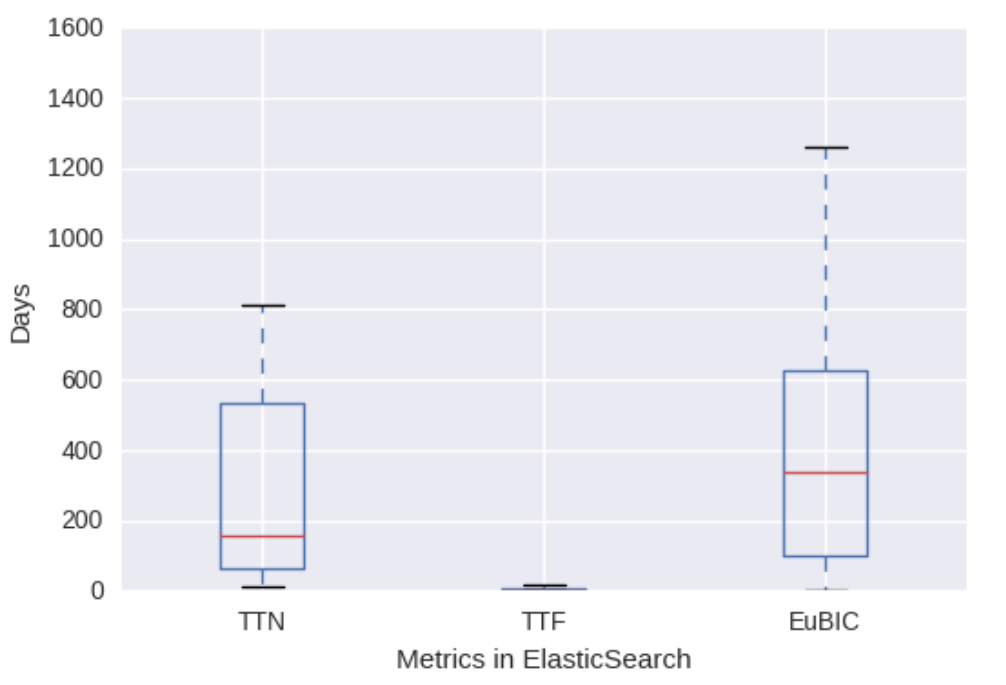
\includegraphics[width=\columnwidth]{boxplotES.png}
\caption{Box-plots with TTN, TTF and EuBIC for the ElasticSearch project.}
\label{fig:meansOfES}       % Give a unique label
%\caption{Box-Plot in ES}
%\label{fig:graph5}       % Give a unique label
\end{figure}

\section{Credibility of SZZ}
\label{sec:Validation}

Prechelt and Pepper offer a good overview of the limitations of the methods to identify BIC's when adopted by practitioners. They point out that one of the obstacles in the way of a reliable analysis are the ``additional changes between defect insertion time and defect correction time that happen to happen at subsequently defect-corrected locations''~\cite{prechelt2014software}. Some methods that consider sources of information other than the previous commit have been proposed already; so, German \emph{et al.}~\cite{german2009change} 
point out that software is in constant change, and that changes performed may have impact across the whole system and may lead to the manifestation of bugs in unchanged parts. In those cases, a bug may emerge in a different location from the source of the bug, which is a change to a function somewhere else in the source code base. 

Hata \emph{et al.} proposed an approach using text features for fault-prone module detection. To identify the faulty modules they used the SZZ algorithm in spite of their knowledge of some limitations such as that incorrect identifications of training data badly influence the quality of the detection or, that an incorrect identification of the test data implies the metrics cannot be calculated properly~\cite{hata2010fault}. In the same line, Mizuno \emph{et al.} use SZZ to identify faulty modules in order to build a model that predict if a change is likely to be a BIC, despite the limitations they described in their paper~\cite{mizuno2010prediction}.

Da Costa \emph{et al.} have made an important effort evaluating the results of five alternative SZZ implementations using a proposed a framework. The evaluation is based on three criteria: (1) the earliest bug appearance, (2) the future impact of changes and, (3) the \emph{realism} of bug introduction, meaning the likelihood that the BIC given by SZZ is the \emph{real} cause of the bug. Their findings show that at least 46\% of the bugs are caused by BIC's that are years apart one from another, suggesting that the current SZZ implementations still lack mechanisms to correctly identify the \emph{real} BIC. Furthermore, they point out to some of the core problems that are not addressed by SZZ and which are addresses in this article, such as finding the BIC when the bugs are fixed by only adding code, or that SZZ may flag potential BIC's that were correct changes at the time of committing~\cite{da2016framework}.

The limitations of the SZZ algorithm are known as the previous paragraphs have showed, but researchers are still using it in their studies. Currently the SZZ algorithm paper has more than 500 cites, to understand how and why researchers have used it, we are working on a systematic review of previous studies that have used this algorithm, with a specific focus on the purpose, methods, and credibility. The review uses more than 400 papers in journals, conference proceedings, workshops and thesis publications. The main goal of this work is to better understand how others use this algorithm and also provide some guidelines to improve the credibility of techniques that are used to locate the origins of the bug.

\section{Conclusion and further research}
\label{sec:conclusions}

In this paper we present two of our ongoing research works, the first describes a new approach to locate the origin of a bug base on the idea of testing each previous version until find the version that causes the malfunction of the code. This way, we could reduce the false positives and also find the missing false negatives that other approach give us. And this empirical study gives cause for understanding how
metrics extracted from the precise location of a bug are related to the maintenance and evolution of a software.

While the second one provides deep insight on the credibility of the most known algorithm to locate the line(s) that injected the bug into the source code. With a systematic review of this algorithm we try to understand how other studies used it and what was their purpose.

A future line could be to perform a detailed research on how this metric could be helpful in defect prediction field, building new models or improving them.

The full automation of the methodology used in this paper is also interesting from a practical point of view. That would provide software projects with a valuable tool for understanding how bugs are introduced, and therefore calculate these metrics for mitigation.
% trigger a \newpage just before the given reference
% number - used to balance the columns on the last page
% adjust value as needed - may need to be readjusted if
% the document is modified later
%\IEEEtriggeratref{8}
% The "triggered" command can be changed if desired:
%\IEEEtriggercmd{\enlargethispage{-5in}}

% references section

% can use a bibliography generated by BibTeX as a .bbl file
% BibTeX documentation can be easily obtained at:
% http://www.ctan.org/tex-archive/biblio/bibtex/contrib/doc/
% The IEEEtran BibTeX style support page is at:
% http://www.michaelshell.org/tex/ieeetran/bibtex/
%\bibliographystyle{IEEEtran}
% argument is your BibTeX string definitions and bibliography database(s)
%\bibliography{IEEEabrv,../bib/paper}
%
% <OR> manually copy in the resultant .bbl file
% set second argument of \begin to the number of references
% (used to reserve space for the reference number labels box)
%\begin{thebibliography}{1}

%\bibitem{IEEEhowto:kopka}
%H.~Kopka and P.~W. Daly, \emph{A Guide to \LaTeX}, 3rd~ed.\hskip 1em plus
%  0.5em minus 0.4em\relax Harlow, England: Addison-Wesley, 1999.

%\end{thebibliography}
%\newpage

\bibliographystyle{abbrv}
\bibliography{sigproc} 


% that's all folks
\end{document}


